\chapter{反三角函数与简单三角方程的解法}
\section{反正弦函数}
我们知道,正弦函数$y=\sin x$是一个周期等于$2\pi$的振动函
数,它的定义域是$(-\infty,+\infty)$, 而值域是闭区间$[-1,1]$, 它的图象如图9.1。

\begin{figure}[htp]
    \centering
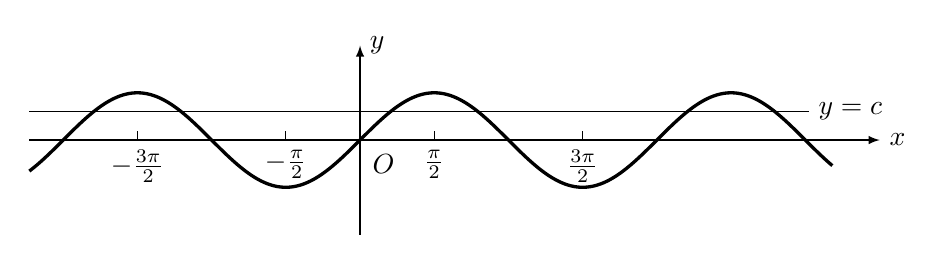
\begin{tikzpicture}[>=latex, scale=.6]
\draw[->] (-7,0)--(11,0)node[right]{$x$};
\draw [->] (0,-2)--(0,2)node[right]{$y$};

\draw[domain=-7:10, samples=1000, very thick] plot(\x,{sin(\x r)});
\draw  (-7,.6)--(9.5,0.6)node[right]{$y=c$};

\foreach \x/\xtext in {-1.5*pi/-\frac{3\pi}{2}, -.5*pi/-\frac{\pi}{2},.5*pi/\frac{\pi}{2}, 1.5*pi/\frac{3\pi}{2}}
{
    \draw (\x,0)node[below]{$\xtext$}--(\x,.2);
}
\node at (.5,-.5){$O$};
\end{tikzpicture}
    \caption{}
\end{figure}


每取一数$y=c,\; -1\le c\le 1$, 作直线$y=c$, 可与正弦曲线
$y=\sin x$交于无穷多个点,这些交点的横坐标是
\[x=x_0+2k\pi\qquad \text{和}\qquad x=(\pi -x_0)+2k\pi\quad (k\in\mathbb{Z})\]
因此有无数多个$x$的值满足方程$\sin x =c$, 而和那个$y=c$对
应。可见对于变数$x$的一切可能实数值来说,我们不能由函
数$f:\mathbb{R}\to [-1,1]$, $f(x)=\sin x$得出它的反函数来。把定
义域分成无数个单调区间,则在各区间$\left[-\frac{\pi}{2}+2k\pi, \frac{\pi}{2}+2k\pi\right]$上,$y=\sin x$由$-1$上升到1,而在各区间$\left[\frac{\pi}{2}+2k\pi, \frac{3\pi}{2}+2k\pi\right]$上,$y=\sin x$由1下降到$-1$,于是由前一章中的
反函数定理知道,对于上述每一个单调区间存在一个反函数。

如果我们强调的是在闭区间$\left[-\frac{\pi}{2},\frac{\pi}{2}\right]$上
来考虑正弦
函数的反函数,我们就说它是反正弦函数的主值,并把这个函数记作
$x=\arcsin y$,使得
$$x=\arcsin y\qquad \Longleftrightarrow \qquad y=\sin x$$
这里$x\in \left[-\frac{\pi}{2},\frac{\pi}{2}\right],\quad y\in[-1,+1]$。

对于使得$y=\sin x$是单调的另一区间,例如$x\in \left[\frac{\pi}{2},\frac{3\pi}{2}\right]$,
我们就得到另一个反正弦函数。假如我们没有明确地
指出反正弦函数的值域所在的区间,我们就不能由函数$y=\sin x$得出它的反函数。为了明确起见,现在我们规定

\begin{blk}{定义1}
    函数$y=\sin x$在闭区间$\left[-\frac{\pi}{2},\frac{\pi}{2}\right]$上
的反函数
叫做\textbf{反正弦函数}或\textbf{反正弦},这个函数用记号写作
$x=\arcsin y$ (即$x$是一角或弧,其相应的正弦值为$y$),
它的定义域是闭区间$-1\le y\le 1$, 值域是闭区间$-\frac{\pi}{2}\le x\le \frac{\pi}{2}$。
\end{blk}

用习惯上的写法,将字母$x$与$y$互换而写成$y=\arcsin x$,
现在,我们将反正弦函数(主值)的定义用几何名词叙述
如下:

在闭区间$-1\le x\le 1$上,数$x$的反正弦$y=\arcsin x$是在
闭区间$\left[-\frac{\pi}{2},\frac{\pi}{2}\right]$上
的一个角或弧,它的正弦值等于$x$, 
即$\sin y=x$.

由反正弦函数的定义和前一章的反函数定理可得到
它的一些性质如下:
\begin{itemize}
    \item $\arcsin(\sin y)=y,\qquad -\frac{\pi}{2}\le y\le \frac{\pi}{2}$
    
    $\sin(\arcsin x)=x,\qquad -1\le x\le 1$

    \item 函数$f(x)=\arcsin x$在闭区间$[-1,1]$上单调递
    增,并且连续。
    \item $y=\arcsin x,\; -1\le x\le 1$的图象与$y=\sin x,\; -\frac{\pi}{2}\le y\le \frac{\pi}{2}$
    的图象关于直线$y=x$对称(图5.2)。
\end{itemize}

\begin{figure}[htp]
    \centering
\begin{tikzpicture}[>=latex, scale=1]
\draw[->] (-4,0)--(4,0)node[right]{$x$};
\draw [->] (0,-3)--(0,3)node[right]{$y$};

\draw[domain=-pi:pi, samples=1000, dashed, thick] plot(\x,{sin(\x r)});
\draw[domain=-1:1, samples=1000, very thick] plot(\x,{asin(\x)*pi/180});
\draw[dashed] (-3,-3)--(2.5,2.5)node [above]{$y=x$};
\draw [dashed] (0,.5*pi)node[left]{$\frac{\pi}{2}$}--(1,.5*pi)node[above]{$y=\arcsin x$};
\draw [dashed] (0,-.5*pi)node[right]{$-\frac{\pi}{2}$}--(-1,-.5*pi);
\node at (.25,-.25){$O$};
\node at (pi+.5,0)[above]{$y=\sin x$};
\foreach \x in {-1,1}
{
    \draw (\x,0)node[below]{$\x$}--(\x,.1);
}
\draw (0,1)node[left]{$1$}--(.1,1);
\draw (0,-1)--(-.1,-1)node[right]{$-1$};

\end{tikzpicture}
    \caption{}
\end{figure}



我们已知正弦函数是奇函数,它的图象关于原点对称,
现在我们要证明 $f(x)=\arcsin x$是奇函数,即
$\arcsin(-x)=-\arcsin x$。

\begin{proof}
    因为$-\frac{\pi}{2}\le \arcsin x\le \frac{\pi}{2}$,
    角$-\arcsin x$也被限制在由$-\frac{\pi}{2}$到$\frac{\pi}{2}$
    的区间内:
    $$-\frac{\pi}{2}\le -\arcsin x\le \frac{\pi}{2}$$
    又,角$-\arcsin x$的正弦等于$-x$
\[\sin(-\arcsin x)=-\sin(\arcsin x)=-x\]
因此:$\arcsin(-x)=-\arcsin x$。
\end{proof}

\begin{example}
    求下列各式的值(口答):
    \begin{enumerate}
        \item $\arcsin\frac{1}{2}$
        \item $\arcsin\left(-\frac{1}{2}\right)$
        \item $\arcsin 1$
    \end{enumerate}
\end{example}

\begin{solution}
\begin{enumerate}
    \item $\arcsin\frac{1}{2}=\frac{\pi}{6}$,因为$\sin\frac{\pi}{6}=\frac{1}{2}$,且$-\frac{\pi}{2}<\frac{\pi}{6}<\frac{\pi}{2}$

    \item $\arcsin\left(-\frac{1}{2}\right)=-\frac{\pi}{6}$,因为$\sin\left(-\frac{\pi}{6}\right)=-\frac{1}{2}$,且
    $-\frac{\pi}{2}<-\frac{\pi}{6}<\frac{\pi}{2}$
    \item $\arcsin 1=\frac{\pi}{2}$,因为$\sin\frac{\pi}{2}=1$,而且$\frac{\pi}{2}$不超出$\left[-\frac{\pi}{2},\frac{\pi}{2}\right]$的界限。
\end{enumerate}
\end{solution}

\begin{example}
    求下列各式的值:
\[\arcsin\left(-\frac{\sqrt{3}}{2}\right),\qquad \arcsin (-0.2672) \]
\end{example}

\begin{solution}
\begin{enumerate}
    \item $\arcsin\left(-\frac{\sqrt{3}}{2}\right)=-\arcsin\frac{\sqrt{3}}{2}=-\frac{\pi}{3}$
    \item $\arcsin(-0.2672)=-\arcsin0.2672=-15^{\circ}30'\approx -0.2705$
\end{enumerate}
    
\end{solution}



\begin{example}
    求下列各式的值:
\begin{multicols}{2}
\begin{enumerate}
    \item $\sin\left(\arcsin\frac{1}{3}\right)$
    \item $\tan\left(\arcsin\frac{\sqrt{2}}{2}\right)$
    \item $\cos\left(\arcsin\frac{3}{5}\right)$
    \item $\sin\left[2\arcsin\left(-\frac{3}{5}\right)\right]$
    \item $\arcsin\left(\sin\frac{7\pi}{6}\right)$
\end{enumerate}
\end{multicols}
\end{example}

\begin{solution}
\begin{enumerate}
    \item $\sin\left(\arcsin\frac{1}{3}\right)=\frac{1}{3}$
    \item $\tan\left(\arcsin\frac{\sqrt{2}}{2}\right)=\tan\frac{\pi}{4}=1$
    \item 设$\arcsin\frac{3}{5}=\alpha$,其中$-\frac{\pi}{2}\le\alpha\le\frac{\pi}{2}$,那么$\sin\alpha=\frac{3}{5}$。由于$-\frac{\pi}{2}\le\alpha\le\frac{\pi}{2}$,$\sin\alpha>0$,可以知道,$\alpha$是第一象限的角,所以
    $$\cos\left(\arcsin\frac{3}{5}\right)=\sqrt{1-\left(\frac{3}{5}\right)^2}=\frac{4}{5}$$
    \item 设$\arcsin\left(-\frac{3}{5}\right)=\alpha$,其中$-\frac{\pi}{2}\le\alpha\le\frac{\pi}{2}$,那么
    \[\sin\alpha =\sin\left[\arcsin\left(-\frac{3}{5}\right)\right]=-\frac{3}{5}\]
由于$-\frac{\pi}{2}\le\alpha\le\frac{\pi}{2}$和$\sin\alpha<0$,可以知道$\alpha$是第四象限的角,所以
\[\cos\alpha=\sqrt{1-\left(-\frac{3}{5}\right)^2}=\frac{4}{5}\]
即:
$\sin\left[2\arcsin\left(-\frac{3}{5}\right)\right]=\sin2\alpha=2\sin\alpha\cdot \cos\alpha=2\left(-\frac{3}{5}\right)\cdot\left(\frac{4}{5}\right)=-\frac{24}{25}$
    \item \[\begin{split}
\arcsin\left(\sin\frac{7\pi}{6}\right)&=\arcsin\left[\sin\left(\pi+\frac{\pi}{6}\right)\right]\\
&=\arcsin\left(-\sin\frac{\pi}{6}\right)\\
&=-\arcsin\left(\sin\frac{\pi}{6}\right)=-\frac{\pi}{6}        
    \end{split}\]
\end{enumerate}
\end{solution}

关于$y=\sin x$, 只要知道了它在闭区间$-\frac{\pi}{2}\le x\le \frac{\pi}{2}$上
的反函数$x=\arcsin y$, 我们便能求出$y=\sin x$在其它单调区间
上的反函数。

\begin{blk}{命题}
\begin{enumerate}
    \item $y=\sin x$在闭区间$\left[-\frac{\pi}{2}+2k\pi,\frac{\pi}{2}+2k\pi\right]$上,由$-1$上升到1,它们相应的反函数是
\[x=\arcsin y+2k\pi,\quad k\in\mathbb{Z}\]
因为
\[\sin x= \sin(\arcsin y+ 2k\pi) = \sin(\arcsin y) = y\]
而且
\[-\frac{\pi}{2}+2k\pi\le \arcsin y+2k\pi \le \frac{\pi}{2}+2k\pi
,\quad k\in\mathbb{Z}\]
    
\item $y=\sin x$在闭区间$\left[\frac{\pi}{2},\frac{3\pi}{2}\right]$上,由1下降到$-1$,
它的反函数是
\[x=\pi-\arcsin y\]
因为
\[\sin x=\sin(\pi- \arcsin y) = \sin(\arcsin y) = y\]
而且
\[\frac{\pi}{2}=\pi-\frac{\pi}{2} \le \pi-\arcsin y \le \pi+\frac{\pi}{2}=\frac{3\pi}{2}\]
我们也可以在单位圆上作图来说明2,如图9.3所示。

\item $y=\sin x$在闭区间$\left[\frac{\pi}{2}+2k\pi,\frac{3\pi}{2}+2k\pi\right]$上,由
1下降到$-1$, 相仿地证得它在相应区间上的反函数是
\[x=(\pi-\arcsin y)+2k\pi,\quad k\in\mathbb{Z} \]
\end{enumerate}
\end{blk}

\begin{figure}[htp]
    \centering
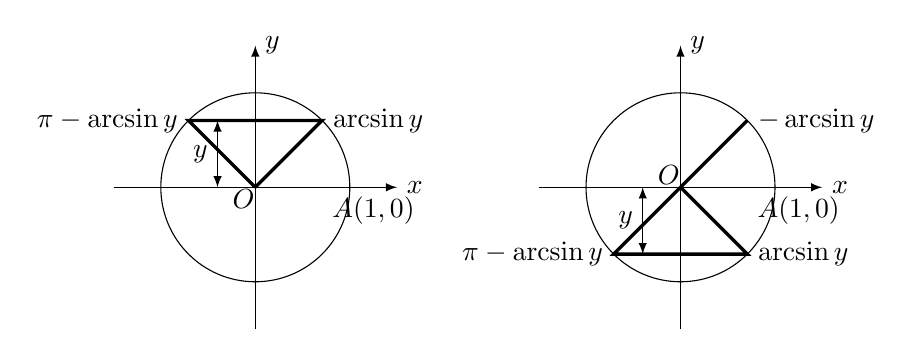
\begin{tikzpicture}[>=latex, scale=.6]
\begin{scope}
    \draw[->] (-3,0)--(3,0)node[right]{$x$};
    \draw[->] (0,-3)--(0,3)node[right]{$y$};
    \draw (0,0) circle(2);
    \node at (-.25,-.25){$O$};
\node at (2.5,0)[below]{$A(1,0)$};
\draw[very thick] (0,0)--(45:2)node[right]{$\arcsin y$}--(90+45:2)node[left]{$\pi-\arcsin y$}--(0,0);

\draw[<->] (-.8,0)--node[left]{$y$}(-.8,1.414);
\end{scope}

\begin{scope}[xshift=9cm]
    \draw[->] (-3,0)--(3,0)node[right]{$x$};
    \draw[->] (0,-3)--(0,3)node[right]{$y$};
    \draw (0,0) circle(2);
    \node at (-.25,.25){$O$};
\node at (2.5,0)[below]{$A(1,0)$};

\draw[<->] (-.8,0)--node[left]{$y$}(-.8,-1.414);
\draw[very thick] (0,0)--(-45:2)node[right]{$\arcsin y$}--(-90-45:2)node[left]{$\pi-\arcsin y$}--(0,0);
\draw[very thick] (0,0)--(45:2)node[right]{$-\arcsin y$};
\end{scope}
\end{tikzpicture}

    \caption{}
\end{figure}


\begin{example}
    讨论函数$y=\arcsin(\sin x)$的图象。
\end{example}

\begin{solution}
    由于正弦的周期性,函数$\arcsin(\sin x),\; x\in\mathbb{R}$也以
$2\pi$为周期,因此,只研究它在长度为$2\pi$的区间内情形即可。
由于
\[\sin y=\sin[\arcsin(\sin x)]=\sin x\]
这里$-\frac{\pi}{2}\le y\le \frac{\pi}{2}$,而$x\in\mathbb{R}$,故
\begin{itemize}
    \item 当$x\in\left[-\frac{\pi}{2},\frac{\pi}{2}\right]$时,则$y=x$。
    \item 当$x\in\left[\frac{\pi}{2},\frac{3\pi}{2}\right]$时,则由上面的命题2知
    \[x=\pi-y\quad \Rightarrow\quad y=\pi-x\in \left(-\frac{\pi}{2},\frac{\pi}{2}\right)\]
\end{itemize}
因之,在此区间内函数的图象与直线$y=\pi-x$一致,总之,
由上面的命题中的1和3的结果:
\begin{enumerate}
    \item 当$x\in \left[-\frac{\pi}{2}+2k\pi,\frac{\pi}{2}+2k\pi\right]$时,则$x=y+2k\pi$,则$y=x-2k\pi$;
    \item 当$x\in \left[\frac{\pi}{2}+2k\pi,\frac{3\pi}{2}+2k\pi\right]$时,则$x=\pi-y+2k\pi$,则$y=(\pi-x)-2k\pi$。
\end{enumerate}
由上面讨论的结果,得到函数$y= \arcsin
(\sin x)$的图象是折线的形状,如图5.4所示。
\begin{figure}[htp]
    \centering
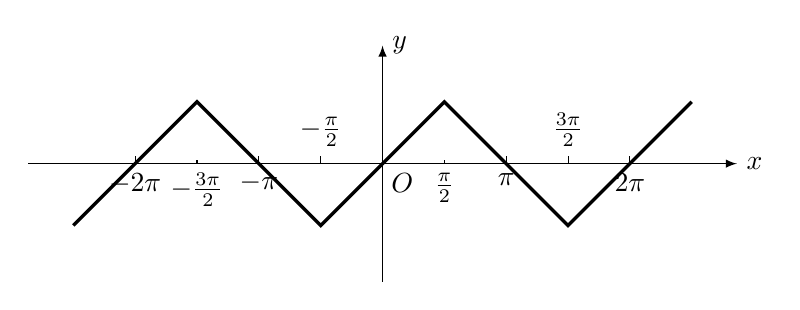
\begin{tikzpicture}[>=latex, scale=.5]
    \draw[->] (-9,0)--(9,0)node[right]{$x$};
    \draw[->] (0,-3)--(0,3)node[right]{$y$};
\draw[very thick] (-2.5*pi,-0.5*pi)--(-1.5*pi,.5*pi)--(-.5*pi,-0.5*pi)--(.5*pi,.5*pi)--(1.5*pi,-0.5*pi)--(2.5*pi,.5*pi);
\foreach \x/\xtext in {-2/-2\pi, -1/-\pi,1/\pi,2/2\pi}
{
    \draw (pi*\x,0)node[below]{$\xtext$}--(pi*\x,0.2);
}
\foreach \x/\xtext in {.5/\frac{\pi}{2},-1.5/-\frac{3\pi}{2}}
{
    \draw (pi*\x,0)node[below]{$\xtext$}--(pi*\x,0.1);
}
\foreach \x/\xtext in {1.5/\frac{3\pi}{2},-.5/-\frac{\pi}{2}}
{
    \draw (pi*\x,0)--(pi*\x,0.2)node[above]{$\xtext$};
}
\node at (.5,-.5){$O$};

\end{tikzpicture}
    \caption{}
\end{figure}
\end{solution}



\section*{习题9.1}
\addcontentsline{toc}{subsection}{习题9.1}
\begin{enumerate}
    \item 用反三角函数表示下面等式中的角。
    \begin{multicols}{2}
\begin{enumerate}
    \item $\sin\frac{\pi}{4}=\frac{\sqrt{2}}{2}$
    \item $\sin\frac{5\pi}{3}=-\frac{\sqrt{3}}{3}$
    \item $\sin\frac{7\pi}{3}=\frac{\sqrt{3}}{2}$
    \item $\sin(-2.314)=-0.04038$
\end{enumerate}
    \end{multicols}
    \item 当$\frac{1}{2}\le x\le\frac{\sqrt{3}}{2}$
    时,求函数$y=x\arcsin x$的最大值
    和最小值。
    \item 不求值,确定下面差的符号:
\begin{enumerate}
    \item $\arcsin 0.7-\arcsin 0.5$
    \item $\arcsin\left(-\frac{3}{5}\right)-\arcsin\left(-\frac{3}{4}\right)$
    \item $\arcsin\left(\sqrt{2}-1\right)-\arcsin\left(\sqrt{5}-2\right)$
\end{enumerate}
\item 求下列各式的值:
\begin{multicols}{2}
\begin{enumerate}
    \item $\arcsin\frac{\sqrt{3}}{2}$
    \item $\arcsin\left(-\frac{\sqrt{2}}{2}\right)$
    \item $\arcsin0$
    \item $\arcsin(-1)$
    \item $\arcsin\left(-\frac{1}{4}\right)$
    \item $\arcsin0.7841$
\end{enumerate}
\end{multicols}

\item 计算下列各式的值:
\begin{multicols}{2}
    \begin{enumerate}
        \item $\tan\left(\arcsin\frac{\sqrt{2}}{2}\right)$
        \item $\cos\left(\arcsin \frac{3}{5}\right)$
        \item $\arcsin \left[\sin\left(-\frac{\pi}{7}\right)\right]$
        \item $\arcsin\left(\sin\frac{5\pi}{6}\right)$
        \item $\arcsin(\cos1)$
    \end{enumerate}
    \end{multicols}
    \item 计算下列各式的值:
\begin{multicols}{2}
    \begin{enumerate}
        \item $\cot\left(2\arcsin\frac{\sqrt{2}}{2}\right)$
        \item $\cos\left(2\arcsin\frac{1}{3}\right)$
        \item $\sin\left(3\arcsin\left(-\frac{\sqrt{3}}{2}\right)\right)$
        \item $\tan\left(\frac{1}{2}\arcsin\frac{2}{3}\right)$
    \end{enumerate}
    \end{multicols}

    \item 讨论函数$y=x \arcsin(\sin x)$的图象,并作草图。
\item 画出$f(x)=\sin(3\arcsin x)$的图象。
\end{enumerate}

\section{反余弦函数}
由余弦函数$y=\cos x$的图象(图9.5)看出,函数$y=\cos x$
在闭区间$[2k\pi ,(2k+1)\pi ]$上,由1下降到$-1$, 而在闭区间
$[(2k-1)\pi ,2k\pi]$上,由$-1$上升到1; 因此,对于上述每一
个单调区间,函数$y=\cos x$都带来一个反函数。

\begin{figure}[htp]
    \centering
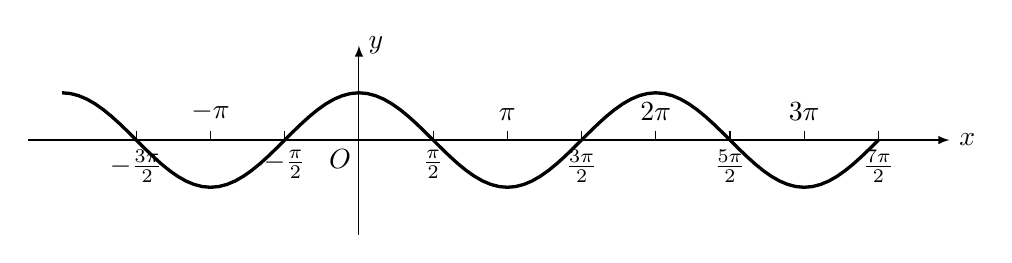
\begin{tikzpicture}[>=latex, scale=.6]
\draw[->] (-7,0)--(12.5,0)node[right]{$x$};
\draw[->] (0,-2)--(0,2)node[right]{$y$};
\foreach \x/\xtext in {-3/-\frac{3\pi}{2},-1/-\frac{\pi}{2},1/\frac{\pi}{2},3/\frac{3\pi}{2},5/\frac{5\pi}{2},7/\frac{7\pi}{2}}
{
    \draw(\x*pi/2, 0)node[below]{$\xtext$}--(\x*pi/2,.2);
}
\foreach \x/\xtext in {-1/-\pi, 1/\pi, 2/2\pi, 3/3\pi}
{
    \draw(\x*pi, 0)--(\x*pi,.2)node[above]{$\xtext$};
}
\draw [domain=-2*pi:3.5*pi, samples=100, very thick]plot(\x, {cos(\x r)});
\node at (-.4,-.4){$O$};
\end{tikzpicture}
    \caption{}
\end{figure}

\begin{blk}{定义2 }
    函数$y=\cos x$在闭区间$[0,\pi]$上的反函数叫做\textbf{反
余弦函数}或\textbf{反余弦},记作
\[x=\arccos y\]
它的定义域是闭区间$[-1,1]$。
\end{blk}

用几何名词来叙述这个定义,便是(互换字母$x$、$y$的
位置):在闭区间$-1\le x\le 1$上,数$x$的反余弦
$y=\arccos x$
是在闭区间$[0,\pi]$的一个角或弧,它的余弦值等于$x$, 即
$\cos y=x$。

\begin{example}
    求下列各式的值(口答):
    \begin{multicols}{2}
\begin{enumerate}
    \item $\arccos\frac{1}{2}$
    \item $\arccos\left(-\frac{1}{2}\right)$
    \item $\arccos1$
    \item $\arccos0$
\end{enumerate}
    \end{multicols}
\end{example}

\begin{solution}
\begin{enumerate}
    \item $\arccos\frac{1}{2}=\frac{\pi}{3}$,因为$\cos\frac{\pi}{3}=\frac{1}{2}$,而且$0<\frac{\pi}{3}<\pi$。
    \item $\arccos\left(-\frac{1}{2}\right)=\frac{2\pi}{3}$,因为$\cos\frac{2\pi}{3}=\cos\left(\pi-\frac{\pi}{3}\right)=\frac{1}{2}$,而且$0<\frac{2\pi}{3}<\pi$。
    \item $\arccos1=0$,因为$\cos 0=1$而且0不出$[0,\pi]$的界限。
    \item $\arccos0=\frac{\pi}{2}$,因为$\cos\frac{\pi}{2}=1$,而且$0<\frac{\pi}{2}<\pi$。
\end{enumerate}
\end{solution}

由反余弦函数的定义和反函数的定理得到反余弦的性质
如下:
\begin{enumerate}
\item $\arccos(\cos y)=y,\; 0\le y\le \pi,\qquad \cos(\arccos x)=x,\; -1\le x\le 1$
\item 函数$f(x)=\arccos x$在闭区间$[-1,1]$上,由$\pi$下
降到0, 且连续。
\item 我们知道互补的两个角$\alpha$和$\pi-\alpha$的余弦是相反
数,即
\[\cos(\pi-\alpha)=-\cos\alpha\]
反之,在区间$[-1,1]$内的相反数的反余弦互为补角,即
\[\arccos(-x)=\pi-\arccos x,\qquad x\in [-1,1]\]

\item 反余弦函数$y=\arccos x$的图象如图9.6所示。
\begin{figure}[htp]
    \centering
\begin{tikzpicture}[>=latex, scale=1.8]
    \draw[->] (-2,0)--(2,0)node[right]{$x$};
    \draw[->] (0,-.5)--(0,3.5)node[right]{$y$};
\draw[domain=-1:1, samples=1000, very thick] plot(\x, {acos(\x)*pi/180});
\node at (.1,-.1){$O$};
\foreach \x/\xtext in {-1/-1,1/1,-.4/-x,.4/x}
{
    \draw (\x,0)node[below]{$\xtext$}--(\x,.1);
}
\node at (0,.5*pi) [right]{$\frac{\pi}{2}$};
\node at (-1,pi) [left]{$y=\arccos x$};
\draw[dashed](-1,0)--(-1,pi)--(0,pi)node[right]{$\pi$};
\draw[dashed](-.4,0)--(-.4,1.98)--(0,1.98)node[right]{$\arccos(-x)$};
\draw[dashed](.4,0)--(.4,1.16)node[right]{$\arccos x$}--(0,1.16);

\end{tikzpicture}
    \caption{}
\end{figure}
\end{enumerate}

\begin{proof}
    因为$0\le \arccos(-x)\le \pi$, 又$0\le \pi -\arccos x\le x$
而且
\[\cos(\pi -\arccos x)=-\cos(\arccos x)=-x\]
由余弦函数在$[0,\pi]$ 上是单调的,得到
\[\pi -\arccos x=\arccos (-x)\]
\end{proof}

\begin{example}
    求下列各式的值:
$\arccos\left(-\frac{\sqrt{2}}{2}\right),\qquad \arccos(-0.9695)$
\end{example}


\begin{solution}
\[\arccos\left(-\frac{\sqrt{2}}{2}\right)=\pi-\arccos\left(\frac{\sqrt{2}}{2}\right)=\pi-\frac{\pi}{4}=\frac{3\pi}{4}\]
\[\begin{split}
    \arccos(-0.9695)&=180^{\circ}-\arccos0.9695\\
    &=180^{\circ}-14^{\circ}11'=165^{\circ}49'\approx 165.82^{\circ}\\
    &\approx 0.9212\pi\approx 2.894\text{弧度}
\end{split}\]
\end{solution}


\begin{example}
求$\tan\left[\arccos\left(-\frac{2\sqrt{2}}{3}\right)\right]$的值。
\end{example}

\begin{solution}
设$\arccos\left(-\frac{2\sqrt{2}}{3}\right)=\alpha$,其中$0\le \alpha\le \pi$,那么,$\cos\alpha=-\frac{2\sqrt{2}}{3}$,由于$0\le\alpha\le \pi$和$\cos\alpha<0$。可以知道$\alpha$是第二象限的角,所以
\[\tan\alpha=-\sqrt{\frac{1}{\cos^2\alpha}-1}=-\sqrt{\frac{9}{8}-1}=-\sqrt{\frac{1}{8}}=-\frac{\sqrt{2}}{4}\]
\end{solution}


\begin{example}
证明:若$|x|\le 1$,则$\arcsin x+\arccos x=\frac{\pi}{2}$

\end{example}

\begin{proof}
 $\because\quad    \sin\left(\frac{\pi}{2}-\arccos x\right)=\cos(\arccos x)=x$

    又    $\sin(\arcsin x)=x$, 且
  \[  0\le \arccos x\le \pi,\qquad -\frac{\pi}{2}\le \frac{\pi}{2}-\arccos x\le \frac{\pi}{2}\]

$\therefore\quad \arcsin x$和$\frac{\pi}{2}-\arccos x$是$\sin x$在单调区间$\left[-\frac{\pi}{2},\frac{\pi}{2}\right]$上的角。

根据$\sin x$在这区间上的单调性,有
$\arcsin x=\frac{\pi}{2}-\arccos x$
即:
\[\arcsin x+\arccos x=\frac{\pi}{2}\]
\end{proof}

\begin{example}
证明:$\arcsin\frac{4}{5}+\arccos\frac{12}{13}+\arcsin\frac{16}{65}=\frac{\pi}{2}$
\end{example}

\begin{proof}
\[\begin{split}
    \arcsin\frac{4}{5}+\arccos\frac{12}{13}&=\frac{\pi}{2}-\arcsin\frac{16}{65}\\
&=\arccos\frac{16}{65}
\end{split}\]
    
令$\alpha=\arcsin\frac{4}{5}$,则$\sin\alpha=\frac{4}{5}$,$0<\alpha<\frac{\pi}{2}$,$\cos\alpha=\frac{3}{5}$。

令$\beta=\arccos\frac{12}{13}$,则$\cos\beta=\frac{12}{13}$,$0<\beta<\frac{\pi}{2}$,$\sin\beta=\frac{5}{13}$。

因此:\[\begin{split}
    \cos(\alpha+\beta)&=\cos\alpha\cos\beta-\sin\alpha\sin\beta\\
    &=\frac{3}{5}\cdot \frac{12}{13}-\frac{4}{5}\cdot \frac{5}{13}=\frac{16}{65}
\end{split}\]

$\because\quad 0<\alpha+\beta<\pi$, $\therefore\quad \alpha+\beta=\arccos\frac{16}{65}$,即:
\[\arcsin\frac{4}{5}+\arccos\frac{12}{13}=\arccos\frac{16}{65}=\frac{\pi}{2}-\arcsin\frac{16}{65}\]

\[\therefore\quad \arcsin\frac{4}{5}+\arccos\frac{12}{13}+\arcsin\frac{16}{65}=\frac{\pi}{2}\]
\end{proof}

在余弦函数的其它单调区间内,其反函数可按下列方式
去找:

\begin{blk}{命题1}
\begin{enumerate}
    \item 在闭区间$[2k\pi ,(2k+1)\pi]$ 上,$y=\cos x$由
    1下降到$-1$, 在这些闭区间上的反函数是
 \[   x=\arccos y+2k\pi \]
    事实上,角$x\in [2k\pi ,(2k+1)\pi]$, 而且它的余弦等于$y$。
    \item 在闭区间$[(2k-1)\pi ,2k\pi]$ 上,$y=\cos x$的反函数
    是
\[    x=-\arccos y+2k\pi \]
    证明相仿。
\end{enumerate}
\end{blk}

\begin{example}
    讨论函数$y=\arccos(\cos x)$的图象。
\end{example}

\begin{solution}
因为$\cos x$的周期是$2\pi$, 函数$\arccos(\cos x)$也是周期函
数,周期是$2\pi$, 且
\[\cos y=\cos[\arccos(\cos x)]\]
即:
$\cos y=\cos x$, 这里$0\le y\le \pi$, $x\in\mathbb{R}$根据上面的命题,
知道:
\begin{enumerate}
    \item 当$x\in[2k\pi ,(2k+1)\pi]$ 时,$x=y+2k\pi$, 即
$y=x-2k\pi$;
\item  当$x\in[(2k-1)\pi ,2k\pi]$ 时,$x=-y+2k\pi$, 即
$y=-x+2k\pi$。
\end{enumerate}
函数$y=\arccos(\cos x)$的图象是折线(图5.7)。

\begin{figure}[htp]
    \centering
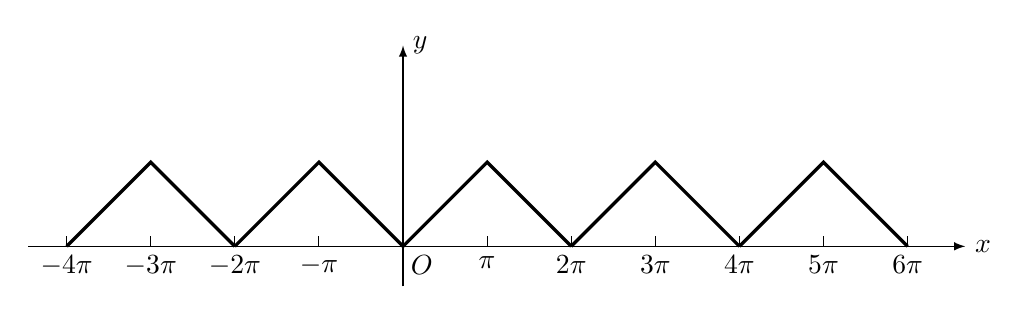
\begin{tikzpicture}[>=latex, scale=.34]
    \draw[->] (-14,0)--(21,0)node[right]{$x$};
    \draw[->] (0,-1.5)--(0,7.5)node[right]{$y$};
\foreach \x in {-4,-2,...,4}
{
    \draw[very thick] (\x*pi,0)--(\x*pi+pi,pi)--(\x*pi+pi+pi,0);
}
\foreach \x in {-4,-3,-2,2,3,4,5,6}
{
    \draw (\x*pi,0)node[below]{$\x\pi$}--(\x*pi,.4);
}
\foreach \x/\xtext in {-1/-\pi,1/\pi}
{
    \draw (\x*pi,0)node[below]{$\xtext $}--(\x*pi,.4);
}
\node at (.7,-.7){$O$};


\end{tikzpicture}    
    \caption{}
\end{figure}
\end{solution}


\section*{习题9.2}
\addcontentsline{toc}{subsection}{习题9.2}

\begin{enumerate}
    \item 用反余弦的形式表示下列各式的角($x\in[0,\pi]$)。
\begin{multicols}{2}
\begin{enumerate}
    \item $\cos\pi =1$
    \item $\cos\frac{5\pi}{3}=-\frac{1}{2}$
    \item $\cos(-3)=-0.9900$
    \item $\cos\frac{7\pi}{6}=-\frac{\sqrt{3}}{2}$
    \item $\cos x=-0.8065$
    \item $\cos x=-1$
\end{enumerate}
\end{multicols}

\item 决定下面差的符号:
\begin{multicols}{2}
\begin{enumerate}
 \item $\arccos0.7-\arccos0.5$
\item $\arccos\left(-\frac{3}{5}\right)-\arccos\left(-\frac{3}{4}\right)$
\item $\arccos\left(\sin\frac{\pi}{12}\right)-\arccos\left(\sin\frac{\pi}{13}\right)$
\end{enumerate}
\end{multicols}
\item 不作计算,确定下列各比的符号:
\begin{multicols}{2}
\begin{enumerate}
    \item $\frac{\arcsin0.85-\arcsin0.8}{\arccos0.85-\arccos0.8}$
    \item $\frac{\pi -2\arcsin(0.9)}{\pi -2\arccos(0.1)}$
    \item $\frac{\arcsin(0.4)+\frac{\pi}{6}}{\arcsin(0.6)-\frac{\pi}{3}}$
\end{enumerate}
\end{multicols}

\item 在同一个坐标系中,作函数$y=\arccos x$
和函数$y=\arccos\frac{x}{2}$
的图象,试根据函数图象说明当$x$为何值时,函数
的差$\arccos\frac{x}{2}-\arccos x$
取最大值、最小值、等于零。
\item 计算下列各式的值:
\begin{multicols}{2}
    \begin{enumerate}
\item $\sin \left(\arccos \frac{1}{2}\right)$
\item $\sin \left(\arccos \frac{3}{5}\right)$
\item $\tan \left(\arccos \frac{5}{13}\right)$
\item $\arcsin (\cos 1)$
\item $\arccos (\cos 2 \pi)$
\item $\arccos \left(-\cos \frac{36}{7} \pi\right)$
\item $\sin \left(\frac{1}{2} \arccos \frac{1}{2}\right)$
\item $\sin \left[3 \arccos \left(-\frac{\sqrt{3}}{2}\right)\right]$
\item $\sin \left[2 \arccos \left(-\frac{2 \sqrt{2}}{3}\right)\right]$
\item $\cos \left(\arcsin \frac{3}{5}-\arccos \frac{5}{13}\right)$    
\item $\sin\left[2\left(\arcsin\frac{\sqrt{5}}{3}-\arccos\frac{\sqrt{5}}{3}\right)\right]$
    \item $\tan\left(\arcsin\frac{1}{2}+\arccos\frac{\sqrt{3}}{2}\right)$
    \end{enumerate}
\end{multicols}

\item 证明下面的恒等式:
\begin{enumerate}
\item 若$0<x<1$, 则:
$\arcsin x=\arccos\sqrt{1-x^2}$
\item 若$0<x<1$, 则:
$\arccos x=\arcsin\sqrt{1-x^2}$
\item 若$-1\le x\le 0$, 则:
$\arcsin x=-\arccos\sqrt{1-x^2}$
\item 若$-1\le x\le 0$, 则:
$\arccos x=\pi-\arcsin\sqrt{1-x^2}$
\end{enumerate}

\item 解下面的方程:
    \begin{enumerate}
\item $\arccos x=\frac{\pi}{3}$
\item $\arccos 2x=0.5$
\item $\arcsin x=\arccos x,\; |x|\le 1$
\item $\arcsin x+\arcsin (1-x)=\arccos x$
\item $\arcsin x-\arccos x=\arcsin (3x-2)$
    \end{enumerate}

\item 当$-\frac{1}{2}\le x\le 0$时,求$f(x)
=\arccos x+x^2$的最小值。
\end{enumerate}

\section{反正切函数}

由正切函数$y=\tan x$的图象(图9.8)可以看出,函数$\tan x$
在每个开区间$\left(-\frac{\pi}{2}+2k\pi, \frac{\pi}{2}+2k\pi\right)$内,由$-\infty$上升到$+\infty$。
所以在每个这样的开区间里能带来一个反函数。


\begin{figure}[htp]
    \centering
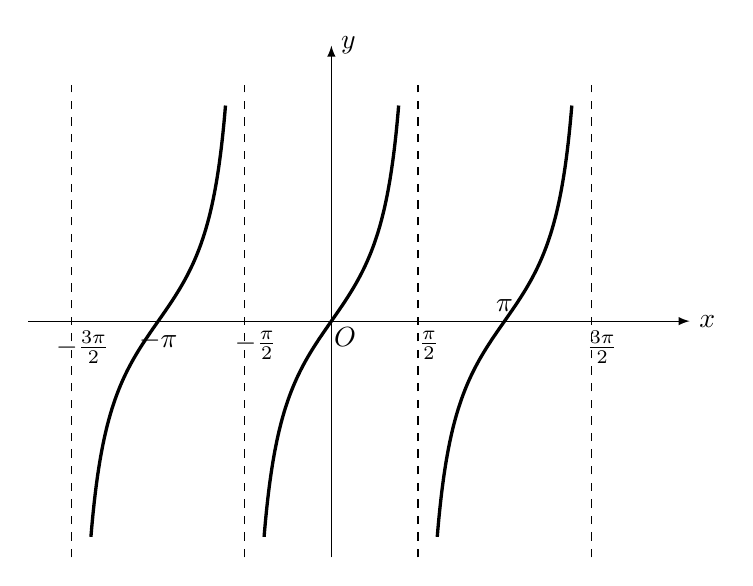
\begin{tikzpicture}[>=latex, xscale=.7]
    \draw[->] (-5.5,0)--(6.5,0)node[right]{$x$};
\draw[->] (0,-3)--(0,3.5)node[right]{$y$};
\foreach \x in {-.5,.5,1.5,-1.5}
{
    \draw[dashed] (\x*pi,-3)--(\x*pi,3);
}

\foreach \y in {-.5,.5,-1.5}
{
    \draw [domain=\y*pi+.35:(\y+1)*pi-.35, samples=1000, very thick] plot(\x, {tan(\x r)});
}

\node at (.25,-.2){$O$};
\node at (-pi,0)[below]{$-\pi$};
\node at (pi,0)[above]{$\pi$};

\node at (-.5*pi+.2,0)[below]{$-\frac{\pi}{2}$};
\node at (.5*pi+.2,0)[below]{$\frac{\pi}{2}$};
\node at (1.5*pi+.2,0)[below]{$\frac{3\pi}{2}$};
\node at (-1.5*pi+.2,0)[below]{$-\frac{3\pi}{2}$};
\end{tikzpicture}
    \caption{}

\end{figure}



\begin{blk}{定义3}
    函数$y=\tan x$在开区间$-\frac{\pi}{2}<x<\frac{\pi}{2}$
内的反函数叫做反正切函数 或 反正
切,记作
\[x=\arctan y\]
因为任何实数都可以作为正
切的值,所以反正切定义域是开区间$-\infty<y<+\infty$
\end{blk}

用几何名词来叙述反正
切的定义就是:在开区间
$(-\infty, +\infty)$内,数$y$的反
正切$x=\arctan y$是在开区间$-\frac{\pi}{2}<x<\frac{\pi}{2}$
内的一个角或弧,它的正切等于$y$,即:$\tan x=y$。

由定义和反函数定理直接得到反正切的性质如下:
\begin{enumerate}
    \item $\arctan (\tan x)=x, \qquad -\frac{\pi}{2}<x<\frac{\pi}{2}$
    
    $\tan (\arctan y)=y,\qquad -\infty<x<+\infty$
    \item $y=\arctan x,\; x\in\mathbb{R}$是单调递增的并且连续;
    \item $\arctan x$是奇函数,即
    \[\arctan (-x)=-\arctan x\]
    证明留给同学们去完成。
    \item 反正切函数$y=\arctan x,\; -\infty<x<+\infty$的图象如
    图5.9所示。
\end{enumerate}

\begin{figure}[htp]
    \centering
\begin{tikzpicture}[>=latex, scale=.7]
    \draw[->] (-5.5,0)--(6.5,0)node[right]{$x$};
    \draw[->] (0,-3)--(0,3)node[right]{$y$};
\draw[dashed] (-5.5,pi/2)--(6.5,pi/2);
\draw[dashed] (-5.5,-pi/2)--(6.5,-pi/2);

\draw [domain=-5.5:5.5, samples=100, very thick]plot(\x, {atan(\x)*pi/180});
\node at (.35,-.35){$O$};
\node at (0,2)[right]{$\frac{\pi}{2}$};
\node at (0,-2)[right]{$-\frac{\pi}{2}$};
\node at (5.5,pi/2-.3)[right]{$y=\arctan x$};
\end{tikzpicture}
    \caption{}
\end{figure}



\begin{example}
    求下列各式的值(口答):
\begin{multicols}{2}
\begin{enumerate}
    \item $\arctan 1$
    \item $\arctan (-1)$
    \item $\arctan \sqrt{3}$
    \item $\arctan (-\sqrt{3})$
\end{enumerate}
\end{multicols}
\end{example}

\begin{solution}
\begin{enumerate}
    \item $\arctan 1=\frac{\pi}{4}$,因为$\tan\frac{\pi}{4}=1$,而且$-\frac{\pi}{2}<\frac{\pi}{4}<\frac{\pi}{2}$
    \item $\arctan (-1)=-\frac{\pi}{4}$,因为$\tan\left(-\frac{\pi}{4}\right)=-1$,而且$-\frac{\pi}{2}<-\frac{\pi}{4}<\frac{\pi}{2}$
    \item $\arctan \sqrt{3}=\frac{\pi}{3}$,因为$\tan\frac{\pi}{3}=\sqrt{3}$,而且$-\frac{\pi}{2}<\frac{\pi}{3}<\frac{\pi}{2}$
    \item $\arctan (-\sqrt{3})=-\frac{\pi}{3}$,因为$\tan\left(-\frac{\pi}{3}\right)=-\sqrt{3}$,而且$-\frac{\pi}{2}<-\frac{\pi}{3}<\frac{\pi}{2}$
\end{enumerate}
\end{solution}

\begin{example}
    求$\cos\left[\arctan\left(-\frac{3}{4}\right)\right]$
\end{example}

\begin{solution}
设$\alpha=\arctan\left(-\frac{3}{4}\right)$,其中$-\frac{\pi}{2}<\alpha<\frac{\pi}{2}$,则$\tan\alpha=-\frac{3}{4}$。

由于$-\frac{\pi}{2}<\alpha<\frac{\pi}{2}$和$\tan\alpha<0$,可以知道$\alpha$是第四象限的角。所以
\[\begin{split}
    \sec\alpha&=\sqrt{1+\tan^2\alpha}=\sqrt{1+\frac{9}{16}}=\frac{5}{4}\\
    \cos\alpha&=\frac{4}{5}
\end{split}\]
就是
\[\cos\left[\arctan\left(-\frac{3}{4}\right)\right]=\cos\alpha=\frac{4}{5}\]
\end{solution}

关于$y=\tan x$在其它单调区间内的反函数,请看下面命题。

\begin{blk}{命题}
    在开区间$\left(-\frac{\pi}{2}+k\pi ,\frac{\pi}{2}+k\pi 
\right)$,$k\in\mathbb{Z}$内$y=\tan x$
由$-\infty$上升到$+\infty$, 在这些区间上的反函数是
$x=\arctan y+k\pi$。
\end{blk}

事实上,$x\in \left(-\frac{\pi}{2}+k\pi ,\frac{\pi}{2}+k\pi 
\right)$而
且
\[\tan x=\tan (\arctan y+k\pi )=\tan (\arctan y)=y\]




\begin{example}
    求$\arctan 2+\arctan 3$的值。
\end{example}

\begin{solution}
    $\because\quad \frac{\pi}{4}=\arctan 1<\arctan 2<\frac{\pi}{2}$,$\frac{\pi}{4}=\arctan 1<\arctan 3<\frac{\pi}{2}$,

    $\therefore\quad \frac{\pi}{2}<\arctan 2+\arctan 3<\pi$。而且
\[\begin{split}
    \tan(\arctan 2+\arctan 3)&=\frac{\tan (\arctan 2)+\tan (\arctan  3)}{1-\tan(\arctan 2)\cdot \tan (\arctan 3)}\\
    &=\frac{2+3}{1-2\x 3}=-1
\end{split}\]
由于$\arctan (-1)\in \left(-\frac{\pi}{2},0\right)$,于是
\[\arctan 2+\arctan 3=\arctan (-1)+\pi=-\frac{\pi}{4}+\pi=\frac{3\pi}{4}\]
\end{solution}

\begin{example}
    讨论 $y=\arctan (\tan x)$的图象。
\end{example}

\begin{solution}
函数$\arctan (\tan x)$的定义域是除去$x=\frac{\pi}{2}+k\pi,\; k\in\mathbb{Z}$
的实数集$\mathbb{R}$, 也就是无数个开区间$\left(-\frac{\pi}{2}+k\pi,\frac{\pi}{2}+k\pi\right),\; k\in\mathbb{Z}$
所组成的一个并集。因此函数$y=\arctan (\tan x)$的图象在
$x=\frac{\pi}{2}+k\pi,\; k\in\mathbb{Z}$这些点处间断。由于
\[\tan y=\tan[\arctan(\tan x)]\]
即:
$\tan y=\tan x$, 这里$-\frac{\pi}{2}<y<\frac{\pi}{2}$, $x\ne \frac{\pi}{2}+k\pi$。

所以,当$x\in\left(-\frac{\pi}{2}+k\pi,\frac{\pi}{2}+k\pi\right)$时,$x=y+k\pi$, 也就是$y=x-k\pi$。于是:
\begin{itemize}
    \item 当$x\in\left(-\frac{\pi}{2},\frac{\pi}{2}\right)$时,$y=x$;
    \item 当$x\in\left(\frac{\pi}{2},\frac{3\pi}{2}\right)$时,$y=x-\pi$;
    \item 当$x\in\left(\frac{3\pi}{2},\frac{5\pi}{2}\right)$时,$y=x-2\pi$;
    \item ………………
    \item 当$x\in\left(-\frac{3\pi}{2},-\frac{\pi}{2}\right)$时,$y=x+\pi$;
    \item ………………
\end{itemize}
现在考虑间断点的情形:

\end{solution}


\begin{example}
    
\end{example}

\begin{solution}
    
\end{solution}


\begin{example}
    
\end{example}

\begin{solution}
    
\end{solution}


\begin{example}
    
\end{example}

\begin{solution}
    
\end{solution}


\begin{example}
    
\end{example}

\begin{solution}
    
\end{solution}


\begin{example}
    
\end{example}

\begin{solution}
    
\end{solution}


\begin{example}
    
\end{example}

\begin{solution}
    
\end{solution}


\begin{example}
    
\end{example}

\begin{solution}
    
\end{solution}


\begin{example}
    
\end{example}

\begin{solution}
    
\end{solution}


\begin{example}
    
\end{example}

\begin{solution}
    
\end{solution}


\begin{example}
    
\end{example}

\begin{solution}
    
\end{solution}


\begin{example}
    
\end{example}

\begin{solution}
    
\end{solution}


\begin{example}
    
\end{example}

\begin{solution}
    
\end{solution}


\begin{example}
    
\end{example}

\begin{solution}
    
\end{solution}


\begin{example}
    
\end{example}

\begin{solution}
    
\end{solution}


\begin{example}
    
\end{example}

\begin{solution}
    
\end{solution}


\begin{example}
    
\end{example}

\begin{solution}
    
\end{solution}


\begin{example}
    
\end{example}

\begin{solution}
    
\end{solution}


\begin{example}
    
\end{example}

\begin{solution}
    
\end{solution}


\begin{example}
    
\end{example}

\begin{solution}
    
\end{solution}


\begin{example}
    
\end{example}

\begin{solution}
    
\end{solution}


\begin{example}
    
\end{example}

\begin{solution}
    
\end{solution}


\begin{example}
    
\end{example}

\begin{solution}
    
\end{solution}


\begin{example}
    
\end{example}

\begin{solution}
    
\end{solution}


\begin{example}
    
\end{example}

\begin{solution}
    
\end{solution}


\begin{example}
    
\end{example}

\begin{solution}
    
\end{solution}


\begin{example}
    
\end{example}

\begin{solution}
    
\end{solution}


\begin{example}
    
\end{example}

\begin{solution}
    
\end{solution}


\begin{example}
    
\end{example}

\begin{solution}
    
\end{solution}


























































































































































